\documentclass[a4paper,11pt]{article}
\usepackage[utf8]{inputenc}
\usepackage{algorithmic}
\usepackage{algorithm}
\usepackage{pst-plot}
\usepackage{graphicx}
\usepackage{endnotes}
\usepackage{graphics}
\usepackage{floatflt}
\usepackage{wrapfig}
\usepackage{amsfonts}
\usepackage{amsmath}
\usepackage{verbatim}
\usepackage{hyperref}
\usepackage{multirow}
\usepackage{pdflscape}
\usepackage{changepage}
\usepackage{environ}
\usepackage{changepage}
\usepackage{caption}
\usepackage{marginnote}
\reversemarginpar

\usepackage{hyperref}
\hypersetup{pdfborder={0 0 0 0}}

% Matlab listing hightlight
\usepackage[T1]{fontenc}
\usepackage[numbered, framed]{matlab-prettifier}
\let\ph\mlplaceholder
\lstMakeShortInline"
\lstset{
  style              = Matlab-editor,
  basicstyle         = \mlttfamily,
  escapechar         = ",
  mlshowsectionrules = true,
}
\DeclareCaptionFormat{listing}{\par\vskip1pt#1#2#3}
\captionsetup[lstlisting]{format=listing,singlelinecheck=false, margin=0pt, font={sf}, labelsep=space, labelfont=bf}

% Page margins and sizes
\pdfpagewidth 210mm
\pdfpageheight 297mm 
\setlength\topmargin{0mm}
\setlength\headheight{0mm}
\setlength\headsep{0mm}
\setlength\textheight{250mm}	
\setlength\textwidth{159.2mm}
\setlength\oddsidemargin{0mm}
\setlength\evensidemargin{0mm}
\setlength\parindent{0mm}
\setlength\parskip{0mm}

% New environments and commands
\NewEnviron{exercise}[3]{\marginnote{
\includegraphics[width=1cm]{brainicon.pdf}\phantom{xx}}[1.2cm]\medskip\paragraph{Exercise #1: #2}\ \\\BODY\ \ \\\phantom{x}\hfill\textbf{\textsc{#3}}\medskip}
\newcommand{\question}[2]{\setlength\parindent{0mm}\ \\$\mathbf{Q_{#1}:}$ #2\ \\}


% Title
\author{\large{Ardi Tampuu, Ilya Kuzovkin, Raul Vicente}}
\title{\huge{Introduction to Computational Neuroscience}\\\LARGE{Introduction to Matlab/Octave}}

\begin{document}
\maketitle

In this course we will use Matlab programming language. The choice is due to the popularity of this language (and the environment) in the neuroscience community. You can use any other programming language if you want to, but some practice session will have basecode in Matlab and data files we will use often come in Matlab format. There are plenty of tutorials online, this practice covers some basics and the most common tasks we will encounter.
\ \\


%
% Introduction
%
\begin{figure}[H]
   \centering
   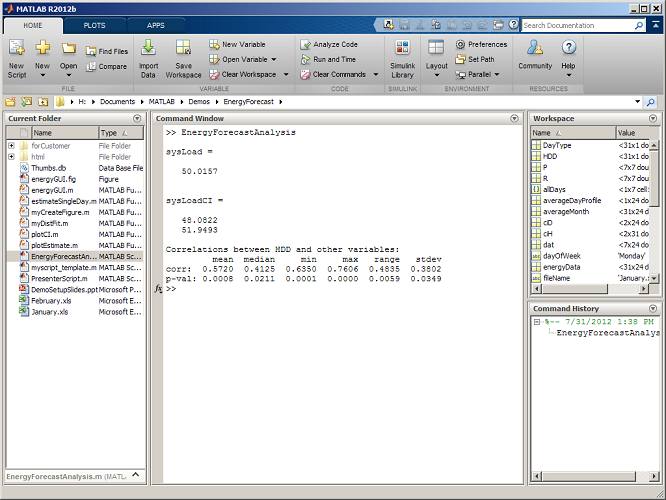
\includegraphics[width=0.95\textwidth]{matlab.png} 
   \caption{Matlab main window}
   \label{fig:matlabgui}
\end{figure}
On Figure \ref{fig:matlabgui} you can see Matlab main window. For Matlab it is very important to know which directory is the current \emph{working directory}. So the first order of business for you is to pick a directory (in the upper part of the screen) where you will complete this practice exercises. Once you unpack the \texttt{01 - Matlab.zip} archive you will have \texttt{01 - Matlab/code} folder in it. I suggest you point Matlab to that folder.\\

The main part of the screen occupies the command line, where you can run you commands. The second essential part of the Matlab is a text editor (which is not shown in default layout). There are also such panels as command log, list of variables in your current workspace and file browser. You can realign the panels to your own liking. The most common way to do work in Matlab is to write you code in editor and sometimes run and test it in the command line.\\

The free alternative to Matlab is called Octave\footnote{Windows: \url{http://wiki.octave.org/Octave_for_Windows} (take the first option: MXE Builds), Mac: \url{http://wiki.octave.org/Octave_for_MacOS_X} (take the binary installer), Linux: distribution packages.}. You can see it on the Figure \ref{fig:octavegui} and there are similar panels available: file browser, list of variables, command history and the command line.

\begin{figure}[H]
   \centering
   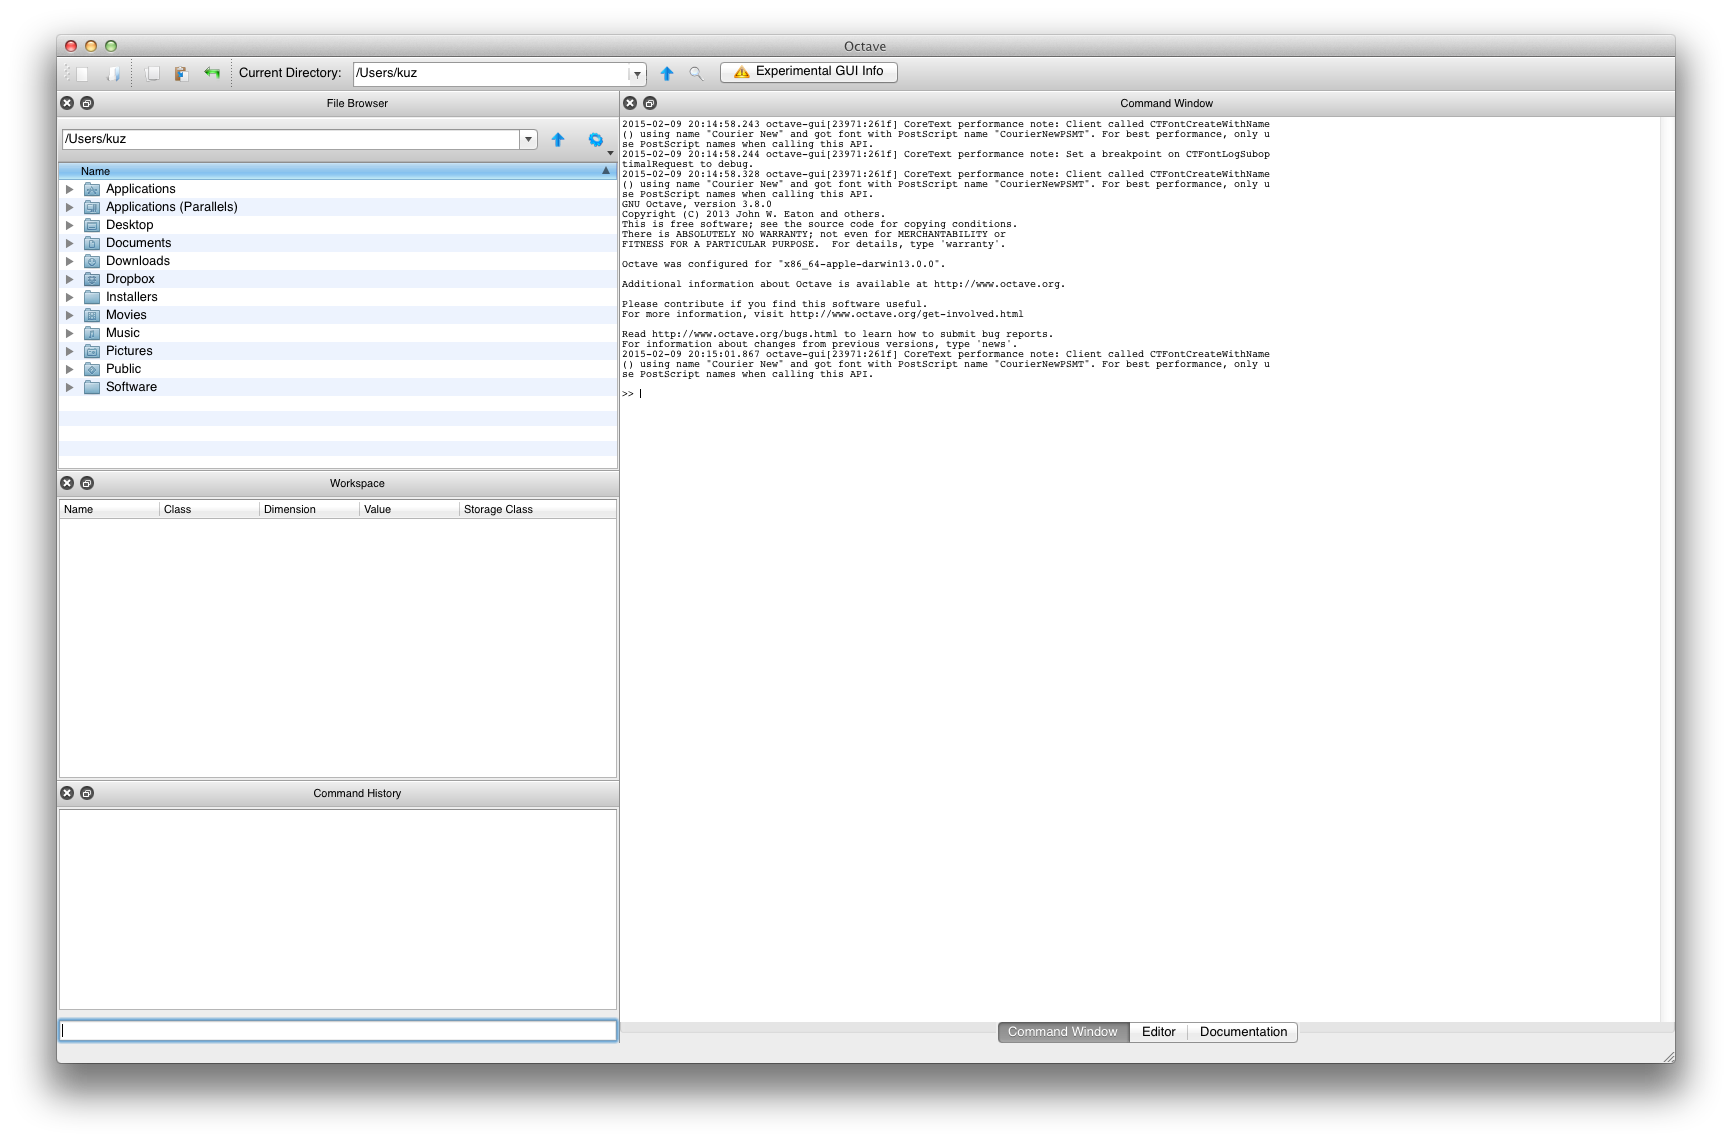
\includegraphics[width=1\textwidth]{octave.png} 
   \caption{Octave main window}
   \label{fig:octavegui}
\end{figure}

Some of the functions in Octave require installing additional packages to use them (somewhat like Matlab Toolboxes). Here is the list of available packages: \url{http://octave.sourceforge.net/packages.php} and here are the instructions how to install: \url{https://www.gnu.org/software/octave/doc/interpreter/Installing-and-Removing-Packages.html}. We will need  \texttt{io} and \texttt{statistics} packages for this tutorial. Once installed a package has to be loaded by calling \texttt{pkg load package\_name}.\\

Now you are all set, we briefly go through basic things you do in any programming language. Read the code and run (copy paste to Matlab/Octave command line) any parts of it which are not immediately clear for you.\\


\textbf{Before you go}: notice that in Matlab/Octave, the indexing starts from 1, not 0. So the first element in an array is at position 1, not position 0 as in many other languages.
\vfill
%
% Language basics
%
\begin{lstlisting}[caption = {Comments}]
% This is a comment, write comments to explain tricky parts of code and outline
% what is happening
\end{lstlisting}

\begin{lstlisting}[caption = {Variables}]
% variable can hold any kind of data, you do not need to specify the type
x = 5;

% semicolon at the end of a line suppresses the output, run and compare
>> x = 5
>> x = 5;

% an array is a bunch of numbers in one variable
v = [1, 2, 3, 4, 5];

% a matrix can be defined as
>> B = [[1, 2, 3]; [4, 5, 6]; [7, 8, 9]; [10, 11, 12]; [13, 14, 15]];
% you can take one element form the matrix by specifying row and column
>> B(1, 1)
% or you can take the whole second row
>> B(2, :)
% or the second column
>> B(:, 2)
% or rows 2, 3, 4 and 5 from columns 2 and 3
>> B(2:5, 2:3)
% to transpose a matrix do
>> B'

% You can also have matrixes with more dimensions than two
>> M = repmat(magic(3), [2, 3, 4, 5]);
% will produce a 4D matrix of size
>> size(M)
ans =     6     9     4     5
% and you can navigate along each dimension, for example
>> M(2, 1, 4, 3)
% which is powerful, but it is easy to loose track of those dimensions, so
% people often use cells

% Cells are most generic stuctures to store anything
>> C = {'here', 'we', 'add', [1, 2, 3, 4, 5], 'whatever we like', 5};
% and then you can access a certain element as 
>> C{4}
ans =     1     2     3     4     5
% indexing starts form 1
\end{lstlisting}
\vfill
\begin{lstlisting}[caption = {Arithmetics}]
% You can add, subtract, multiply, divide numbers
>> 2 + 3 - 4 * 5 / 6
% raise them to power
>> 2^8
% add and subtract vectors
>> [1, 2, 3] + [4, 5, 6] - [7, 8, 9]
% multiply and divide vectors element-wise
>> [1, 2, 3] .* [4, 5, 6] ./ [7, 8, 9]
% multiply matrices
>> [[1, 2]; [3, 4]] * [[5, 6]; [7, 8]]
\end{lstlisting}

\begin{lstlisting}[caption = {\texttt{IF - THEN - ELSE}}]
number = 1;
if number == 1               % as you can see comparison is done using ==
  disp('The number is one')  % this way you can produce output messages
elseif number == 2
  disp('The number is two')
else
  disp('The number is something else')
end
\end{lstlisting}

\begin{lstlisting}[caption = {Loops}]
% FOR loop is the main guy
for i = 1:100
  disp(i)
end

% it can also go over elements in a variable (the 'foreach' behaviour)
C = {'here', 'we', 'add', [1, 2, 3, 4, 5], 'whatever we like', 5};
for c = C
  disp(c{1})
end

% the WHILE loop is also available
i = 0;
while i < 5
    disp(i)
    i = i + 1;
end

% it is often much more efficient to use vectorised code instead of loops
% for example to raise numbers 1 to 100 to power 2 and sum them we can do
total = 0;
for i = 1:100
  total = total + i^2;
end
disp(total)
% but the Matlab way to do it is
total = sum([1:100] .^ 2)
\end{lstlisting}

You will see weird functions now and then, like this \texttt{sum} in the last example. And you may wonder \emph{what does it do exactly?}. To answer that there is a Matlab documentation \url{http://se.mathworks.com/help/} where you can enter \texttt{sum} and read all about it. Or just Google "matlab sum" or "octave sum"

\begin{lstlisting}[caption = {Creating a function, file \texttt{dothings.m}}]
% Each function in Matlab lives in a separate file (you can have several
% functions in one file, but only the first one will be callable from the outside)
% So this is an example of a function, which should be saved as
% a separate file 'dothings.m'

% Matlab function can return several values (in this case four)
function [s, d, p, q] = dothings(a, b)
  s = a + b;
  d = a - b;
  p = a * b;
  q = a / b;
end
% this function will compute sum, difference, product and quotient of two
% numbers a and b
\end{lstlisting}

\begin{lstlisting}[caption = {Calling a function}]
% Now once we have our function defined and saved we can call it
>> [s, d, p, q] = dothings(10, 20)
\end{lstlisting}


%
% Exercise 1
%
\begin{exercise}{1}{Language basics}{}
Write a function which multiplies two matrices $A$ and $B$ and returns the resulting matrix as an output. If matrix dimensions do not match your program should output appropriate message.
\end{exercise}

%\hline

%
% Data
%
\begin{lstlisting}[caption={Working with data},label={lst:data}]
% There are two great functions in Matlab: 'save' and 'load'.
% Suppose you have very important piece of information
>> important = 'I had a cookie today';
% and you want to save it
>> save('mydata.mat', 'important')
% it will save the variable 'important' into file named 'mydata.mat'
>> clear important     % deletes our variable
>> load('mydata.mat')  % loads it back
>> important           % will print out the content of the variable

% load() can also deal with formats other that .mat, such as .csv or .dat
>> load ../data/erptrials.csv % assuming 01 - Matlab/code is working directory
% will load a matrix in your workspace
>> size(erptrials)
ans =          79        2000
% where we have 79 recordings of neural data 2000 data points per each
\end{lstlisting}


%
% Exercise 2
%
\begin{exercise}{2}{Manipulating data}{}
Load the \texttt{erptrials.csv} dataset as described in Listing \ref{lst:data}. Create a subsample of observations by taking first 30 rows (and all of the columns) of the \texttt{erptrials} matrix. Save the resulting matrix of size $30 \times 2000$ as \texttt{one.mat} file. The remaining 49 samples save as \texttt{two.mat}. Use \texttt{clear} command to remove both subsets from your workspace. Now load them both back using \texttt{load}. Glue two subsets together to be one whole set as it was before. Assuming that the original dataset is called \texttt{erptrials} and the resulting one is called \texttt{reconstructed} confirm that they are identical by running \texttt{all(erptrials(:)==reconstructed(:))}.
\end{exercise}


%
% Plotting
%
\begin{lstlisting}[caption={Plotting}]
% One of the most important abilities in any data analysis task is the ability to
% visualise the results.

% generate some a random vector
>> data = rand(1, 100) * 10;

% the simplest way to plot is
>> plot(data)

% there are various ways to plot your data depending on what you have there
>> bar(data)
>> hist(data)

% for two dimensional data
>> data = rand(100, 100) * 10;
% you might find useful
>> area(data)
>> imagesc(data)
>> boxplot(data(:, 1:20))
>> scatter(data(1, :), data(2, :))
% etc...

% by the way if some operation is taking too long you can interrupt
% it by pressing Ctrl + C

% By default Matlab will create one canvas (called figure) and plot everything
% on it, if you want to produce several plots and open them each separately you
% should call 'figure(N)' before each one
>> figure(1)
>> plot(data(1, :))
>> figure(2)
>> plot(data(2, :))

% You can also put several plots onto one canvas
>> subplot(3, 2, 1)
% will create a grid with 3 rows and 2 columns and will plot the next picture
% into cell 1 on this grid
>> plot(data(1, :))
% next we want to put into the second cell
>> subplot(3, 2, 2)
>> plot(data(2, :))
% and so on (better done with a FOR cycle)
>> subplot(3, 2, 3)
>> plot(data(3, :))
>> subplot(3, 2, 4)
>> plot(data(4, :))
>> subplot(3, 2, 5)
>> plot(data(5, :))
>> subplot(3, 2, 6)
>> plot(data(6, :))

\end{lstlisting}


%
% Exercise 3
%
\begin{exercise}{3}{Plotting}{}
Create a plot of 17th row (all columns) of our \texttt{erptrials} dataset. Do you understand what your plot demonstrates? Go through \texttt{plot} function documentation \footnote{\url{http://se.mathworks.com/help/matlab/ref/plot.html}}\footnote{\url{https://www.gnu.org/software/octave/doc/interpreter/Two_002dDimensional-Plots.html}} and make the following changes to your plot:
\begin{itemize}
    \item Add caption, so that everybody would know what this plot is about
    \item Set X-axis label (try to guess what it is or come up with something)
    \item Set Y-axis label (try to guess what it is or come up with something)
    \item Change the color of the line
    \item Change the type of the line
\end{itemize}
\end{exercise}



\end{document}










